\clearpage{\pagestyle{empty}\cleardoublepage}

\chapter{Searches for vector-like top partner pairs in the single lepton channel}~\label{chap:vlq}

Starting from this chapter, and continuing in Chapter~\ref{chap:wbx} 
and Chapter~\ref{chap:htx}, we are going to describe two preliminary 
searches for vector-like top partners \TTbar\ pairs performed in the single 
lepton\footnote{From now on, with the word ``lepton'' we will 
mean only either electron or muon, assumed to come from the leptonic
decay of a $W$ boson with its associated neutrino, which is considered
to be the only particle contributing to the transverse missing energy \met.} channel. 
These analyses
are optimized for different final states and are thus complementary.
The analyses are performed using a partial dataset of the p-p collisions at the \cme\ 
of \rts=8~\tev\ collected during 2012 at the ATLAS detector, consinsting in  14.3~\ifb.
The first search focuses on  vector-like top partners decay channels with high 
Branching Ratio (BR) to 
a $W$ boson and a bottom quark, while the second search is optimized for events with 
high BR to a Higgs boson and a top quark.
%and is performed using the full dataset of p-p collisions at the \cme of \rts=8~\tev\ collected during 2012 at the ATLAS detector, consinsting in 20.34~\ifb, while
%search for vector-like top partners with high BR to $Ht$
%uses a partial dataset of the same data, amounting to 14.3~\ifb.

This chapter is devoted to the presentation of the general features that are common to 
the two analyses and is organized as follows: first in Section~\ref{sec:strategy}
we review the common strategy adopted in the ATLAS collaboration Exotics group
for vector-like quark searches; Section~\ref{sec:presel}
summarises the common event preselection for data and few general concepts in the
analyses design; Section~\ref{sec:MCbkg}
presents the Monte Carlo samples used in the searches, which
are in general common to both analyses with only few exceptions that are reported;
Section~\ref{sec:qcdbkg} describes how the multi-jet background from QCD events is
obtained; Section~\ref{sec:systematics} introduces the general treatment of systematics.
The two analyses are then presented in details in Chapeter~\ref{chap:wbx} 
(\TTbar\ pairs decaying to $Wb+X$) and in Chapter~\ref{chap:htx}
(\TTbar\ pairs decaying to $Ht+X$). The final results are presented 
in Chapter~\ref{chap:results}.

\section{General strategy for vector-like quark pairs searches}\label{sec:strategy}

The phenomenology for vector-like quarks was described already in Section~\ref{sec:THvlq}
of this dissertation, here we will only briefly re-introduce the concepts on which
the strategy for the searches has been built. Table~\ref{tab:vlqdecays} collects the 
decay modes for vector-like quarks in the singlet and doublet models. It is evident
from the richness of the final state phase space, combined with the unpredicted mass
of the heavy objects that could span from few hundreds of \gev s (down to the values exluded by
previous searches) up to  order of one \tev\ (since we focus on pair production of vector-like
quarks, which is favoured up to this mass scale as shown in Figure~\ref{fig:vlqxsec}), that is 
impossible to cover it with a single inclusive search.

\begin{table}[htb]\centering
\begin{tabular}{|lc|lc|}\toprule
\hskip2ex VLQ &  Decay & \hskip2ex VLQ  & Decay \\ 
\hskip1ex Singlets &  modes & \hskip1ex Doublets & modes\\
& & &\\
$T(+2/3)$ & $W^+b,\, Ht,\, Zt$ & \multirow{2}{*}{$\quad\bigg(\begin{array}{c}T \\ B\end{array}\bigg)$} & $W^+b,\, Ht,\, Zt$\\ 
& & & $ W^-t,\, Hb,\, Zb$\\
$B(-1/3)$ & $ W^-t,\, Hb,\, Zb$ & & \\
& & \multirow{2}{*}{$\quad\bigg(\begin{array}{c}T \\ X\end{array}\bigg)$} & $Ht,\, Zt$\\
$X(+5/3)$ & $W^+t$ & & $W^+t$\\
& & &\\
$Y(-4/3)$ & $W^-b$ & \multirow{2}{*}{$\quad\bigg(\begin{array}{c}B \\ Y\end{array}\bigg)$} & $Hb,\, Zb$\\
& & & $W^-b$\\\bottomrule
\end{tabular}
\caption{Allowed decay modes for vector-like singlets and doublets.}\label{tab:vlqdecays}
\end{table}

\begin{figure}[htb]\begin{center}
	\subfigure{
  	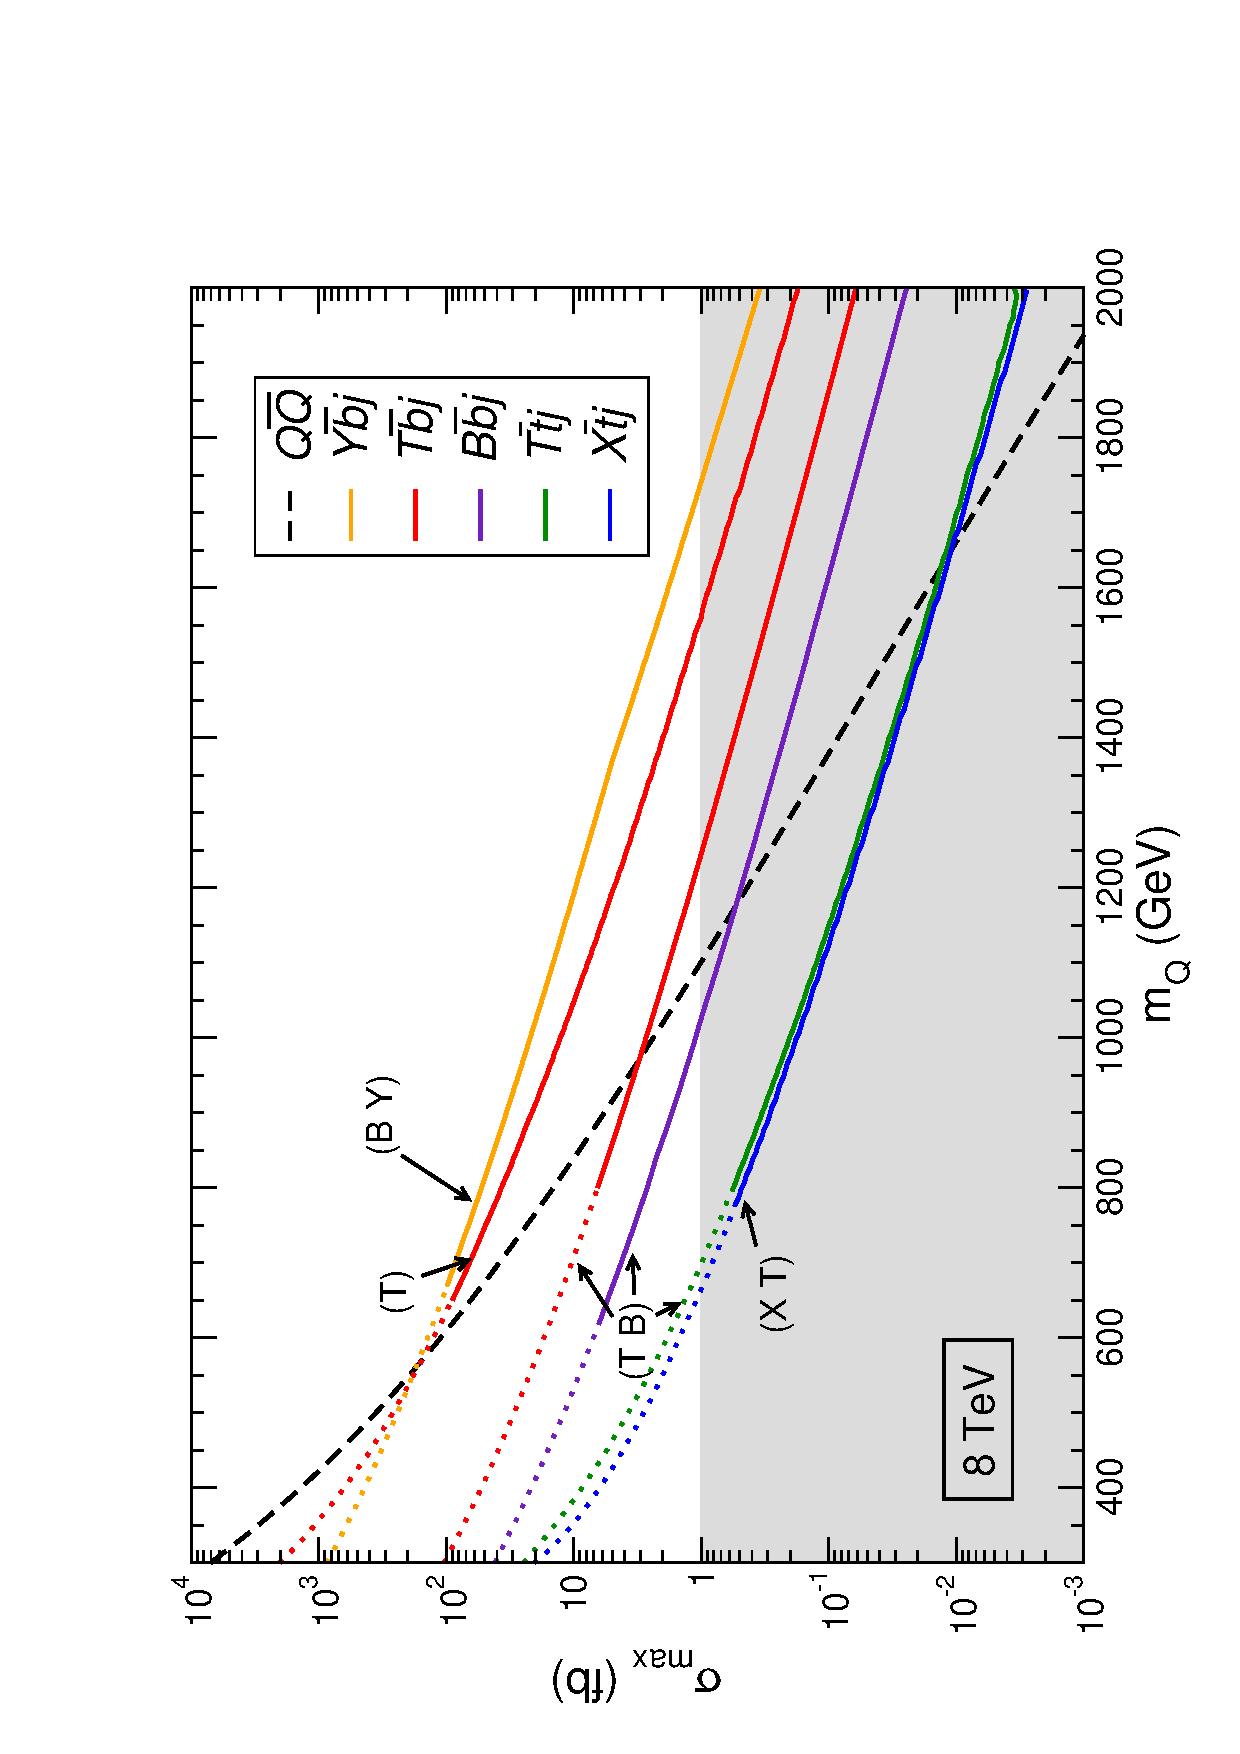
\includegraphics[width=0.65\textwidth, angle=270]{vlq_analysis/figures/xsec-8}}
	\caption{\label{fig:vlqxsec} Pair and single production cross sections  for heavy 
        quarks in proton-proton collisions at $\sqrt{s}=8$~TeV~\cite{Aguilar-Saavedra:2013qpa}.}
\end{center}\end{figure}

The BR of vector-like top and bottom partners to the allowed decay modes depends
on the mass of the heavy quark and on the considered model (in our case, singlet or doublet
scenario), as shown in Figure~\ref{fig:vlqBRs}.
Each decay mode has specific features that allow to define powerful, optimized searches.
Therefore in order to exploit this opportunity and at the same time stay as model independent
as possible, different searches for vector-like quarks are performed at ATLAS
to be later combined, each of them sensitive to specific channels.
To ensure a comprehensive coverage of the phase space, a two-dimensional plane is defined 
(Figure~\ref{fig:2dplane}) as follows:
along the Y axes is the BR of the decay 
modes with a Higgs boson in the final state; along the X axis is the BR 
of the decay modes with a $W$ boson in the final state.
The BR to the channel with a $Z$ boson in the final state is then fixed by the 
unitarity requirement BR($T/B\to  Zt/b$) = 1 - BR($T/B\to Ht/b$) - BR($T/B\to Wb/t$).
A plane of this kind is defined for every vector-like quark mass point considered 
in the analysis. Each point of each plane therefore represents a 
uniquely defined model, and analyses are performed for every configuration
to either find deviations from expectations or to set a 95\% Confidence Level (CL) exclusion.
The final objective of the joint strategy is to cover the full plane.

\begin{figure}[h!tb]\begin{center}
	\subfigure[]{\label{fig:vltBRs}
  	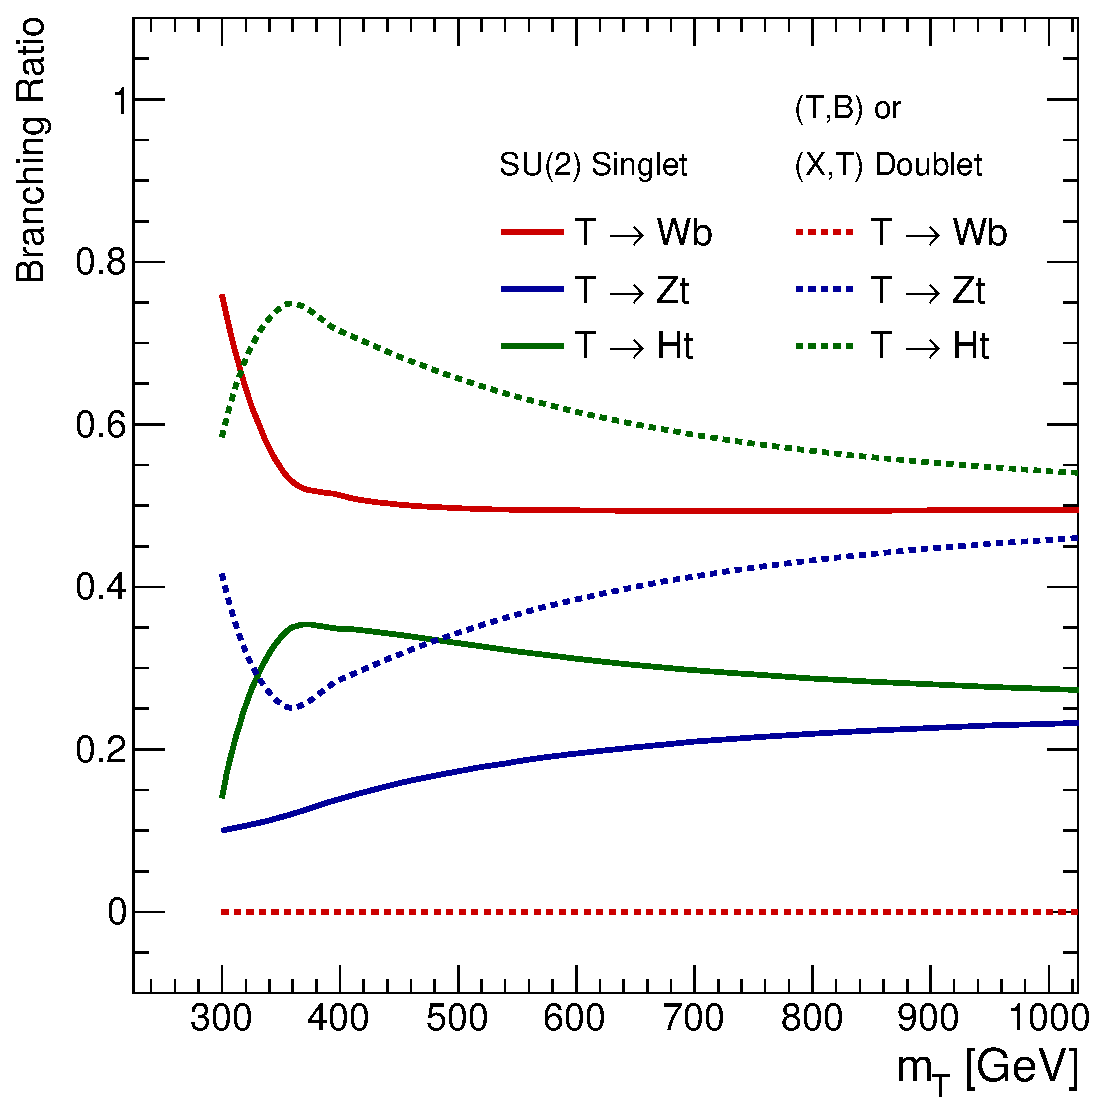
\includegraphics[width=0.47\textwidth]{vlq_analysis/figures/fig_02a.eps}}
	\subfigure[]{\label{fig:vlbBRs}
  	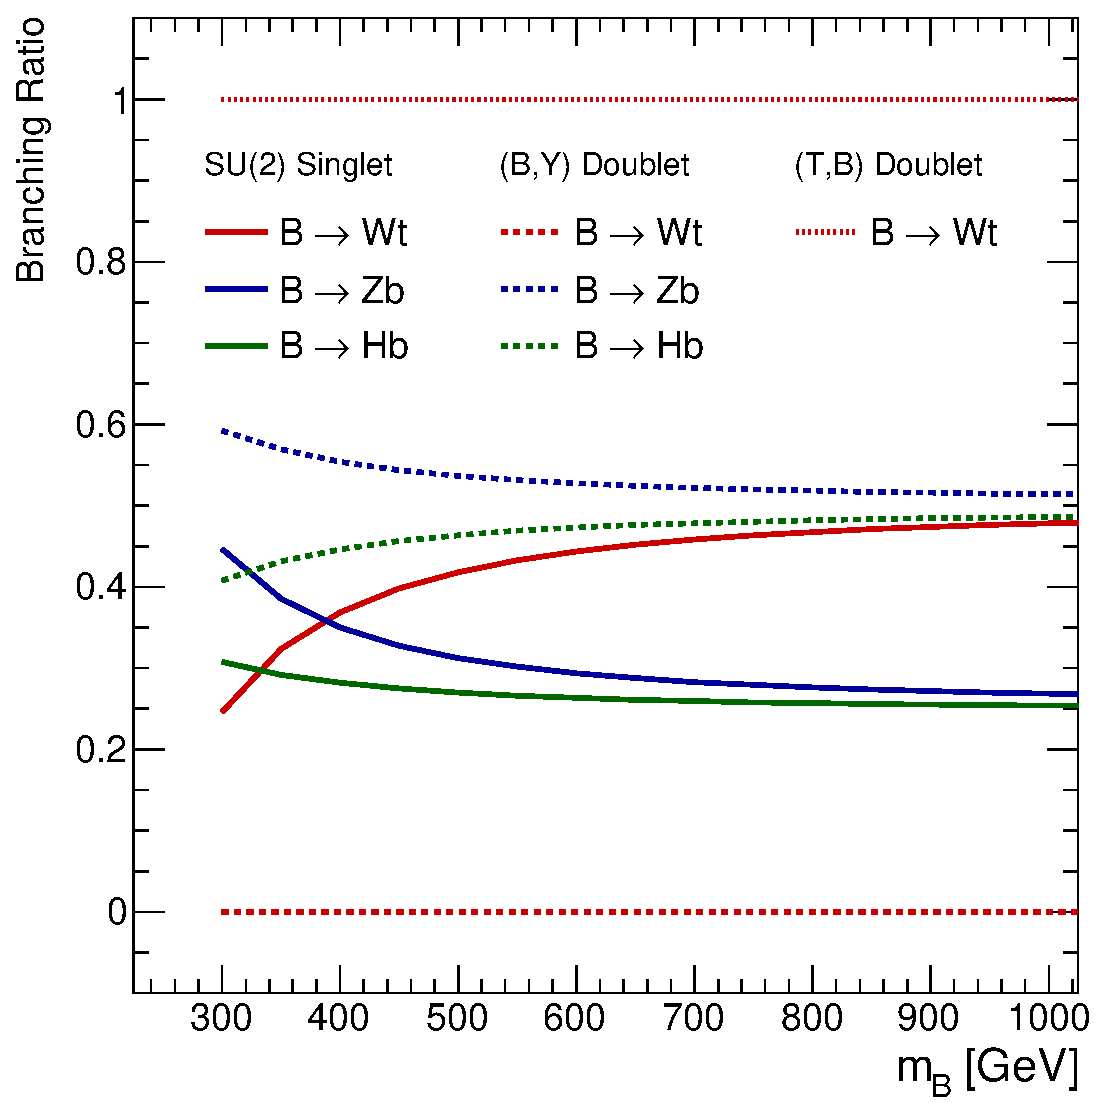
\includegraphics[width=0.47\textwidth]{vlq_analysis/figures/fig_02b.eps}}
	\caption{Branching ratio of vector-like top (a) and bottom (b) partners as a function of the heavy quark mass $m_T$ and $m_B$ respectively~\cite{ATLAS-CONF-2013-056} for singlet and doublet models.\label{fig:vlqBRs}}
\end{center}\end{figure}

\begin{figure}[htb]\begin{center}
	\subfigure{
        \begin{pgfpicture}{0.0\textwidth}{0.0\textheight}{.5\textwidth}{.5\textwidth}
%\begin{pgfpicture}{0.0\textwidth}{0.0\textheight}{1.\textwidth}{.6\textwidth}

\begin{pgfscope}
\pgfsetendarrow{\pgfarrowlargepointed{6pt}}
\pgfsetlinewidth{1.5pt}

\begin{pgftranslate}{\pgfpoint{0.05\textwidth}{0.05\textheight}}
%\begin{pgftranslate}{\pgfpoint{0.1\textwidth}{0.15\textheight}}
  {
    %\color{black}
    \color{black!50!red}
    \pgfputat{\pgfxy(3.5,-0.5)}{\pgfbox[left,base]{BR($T\to Wb$)}}
  }
  {
    \color{black!50!blue}
    \pgfputat{\pgfxy(3.5,-0.8)}{\pgfbox[left,base]{BR($B\to Wt$)}}
  }
  {
    \begin{pgfrotateby}{\pgfdegree{90}}
      {
        \color{black!50!red}
        \pgfputat{\pgfxy(3.5,0.4)}{\pgfbox[left,base]{BR($T\to Ht$)}}
      }
      {
        \color{black!50!blue}
        \pgfputat{\pgfxy(3.5,0.7)}{\pgfbox[left,base]{BR($B\to Hb$)}}
      }
    \end{pgfrotateby}
  }
  {
    \pgfsetlinewidth{1.5pt}
    \color{gray!30!white}%\color{light-gray}
    \pgfmoveto{\pgfxy(5,0)}
    \pgflineto{\pgfxy(5,5)}
    \pgflineto{\pgfxy(0,5)}
    %\pgfstroke
    \pgffill
  }
  {
    %\color{black}
    \pgfputlabelrotated{0.5}{\pgfxy(0,5)}{\pgfxy(5,0)}{8pt}{\pgfbox[center,base]{Forbidden}}
  }
  \begin{pgfscope}
    \pgfmoveto{\pgfxy(5,0)}
    \pgflineto{\pgfxy(0,0)}
    \pgflineto{\pgfxy(0,5)}
    {
      \color{yellow!30!white}
      \pgfclip
      \pgfcircle[fill]{\pgfxy(.5,4)}{35pt}
    }
    {
      \pgfputat{\pgfxy(0.15,3.6)}{\pgfbox[left,base]{\large{\color{black!70!red}$Ht$}{\color{black!70!blue}$(b)$}}}
    }
    {
      \color{yellow!30!white}
      \pgfcircle[fill]{\pgfxy(.6,.6)}{35pt}
    }
    {
      \pgfputat{\pgfxy(0.15,.4)}{\pgfbox[left,base]{\large{\color{black!70!red}$Zt$}{\color{black!70!blue}$(b)$}}}
    }
    {
      \color{yellow!30!white}%\color{light-gray}
      \pgfcircle[fill]{\pgfxy(4,0)}{35pt}
    }
    {
      \pgfputat{\pgfxy(3.2,0.4)}{\pgfbox[left,base]{\large{\color{black!70!red}$Wb$}{\color{black!70!blue}$(t)$}}}
    }
  \end{pgfscope}
  {
    %\color{black}
    \pgfsetendarrow{\pgfarrowlargepointed{6pt}}
    \pgfsetlinewidth{1.5pt}
    \pgfline{\pgfxy(0,0)}{\pgfxy(5.5,0)}
    \pgfstroke
    %\pgfsetendarrow{\pgfarrowlargepointed{6pt}}
    %\pgfsetlinewidth{1.5pt}
    \pgfline{\pgfxy(0,0)}{\pgfxy(0,5.5)}
    \pgfstroke
  }

\end{pgftranslate}
\end{pgfscope}
\end{pgfpicture}
}
       	\caption{Two dimensional plane used to represend the comprehensive scan of model mixing. Searches 
        with a Higgs boson in the final state cover the top left corner; searches with a $Z$ boson in the 
        final state cover the bottom left corner; searches with a $W$ boson in the final state cover the 
        bottom right corner. The shaded area labelled as ``forbidden'' is the unphysical region where
        BR($T/B\to Ht/b$) + BR($T/B\to Wb/t$) + BR($T/B\to  Zt/b$) $>1$ \label{fig:2dplane}}
\end{center}\end{figure}


Up to the date of the writing of this dissertation, four complementary 
and quasi model-independent analyses have been performed by the Exotics working
group on the partial dataset of 14.3~\ifb\ of proton-proton collision data at 
$\sqrt{s}=8\tev$.  
Two analyses investigated dilepton channels, one requiring a pair of same-charge 
leptons~\cite{ATLAS-CONF-2013-051}, 
the other a pair of opposite-charge leptons~\cite{ATLAS-CONF-2013-056}. These two analyses 
are sensitive to
both vector-like top and bottom partners, and the first in particular is also 
sensitive to four-top production $pp\to t\bar{t}t\bar{t}$, 
either through the Standard Model process or a beyond-SM source such as 
pair production of scalar color-octets (sgluons) or gluinos, with subsequent decays to top quark pairs.
While the first search approach is to select via restrictive cuts the eventual signal
and compare the final counts with the expected yields from background sources, the
second search focuses on reconstructing the $Z$ boson from the opposite-charge  lepton
pair and uses the invariant mass of the $Z$ boson candidate paired  with the highest $p_T$ $b$-jet
as final discriminant variable to perform the statistical analysis.

We will in the following treat in details the two searches for vector-like 
top partners performed in the single lepton channels, starting with the
discussion of the common features between the two analyses.


\section{Data sample and common event preselection}\label{sec:presel}

The data from p-p collision events recorded at the ATLAS experiment during
2012 at a \cme\ of $\rts=8\tev$ are considered. Physics object definitions 
were previously discussed in Chapter~\ref{chap:objects}.
Events collected during
stable beam periods are required to pass data quality requirements and
single lepton trigger selection. In order to maximize trigger
efficiency, different transverse momentum threshold triggers are combined
through a logical \OR, with the lower \pt\ ones including isolation requirements
that result in inefficiencies for high \pt\ lepton candidates, recovered with
the use of the higher threshold triggers. The electron triggers have
\pt\ thresholds of 24 and 60~\gev, the muon ones of 24 and 36~\gev\ (Section~\ref{sec:REQtrigger}).

After passing trigger requirements, events with more than one lepton are
discarded. In addition, the only lepton of the event has to match within $\dr<0.15$ the
triggered one. As basic preselectio, four jets satisfying the conditions
described in Section~\ref{sec:jets} are required, at least one of them
being tagged as a \bjet.

In order to suppress the multi-jet background from QCD processes,
combined cuts on the \met\ and on the tranverse mass of the 
leptonically decaying $W$ boson \mt\footnote{$\mt = \sqrt{2 p^\ell_{\rm T} \met (1-\cos\Delta\phi)}$, with
$p^\ell_{\rm T}$  being the transverse momentum (energy) of the muon (electron) and $\Delta\phi$ the
azimuthal angle separation between the lepton and the direction of
the missing transverse momentum.}\ 
are defined: $\met>20~\gev$ and $\met+\mt>60~\gev$.

At this point, a simple consideration about the typical expected jet
(and \bjet) multiplicity is made so as to define an orthogonality
cut between the two analyses. Table~\ref{tab:jetmult} shows the 
number of jets (\bjet s) per decay channel combinations of \TTbar\ pairs, 
in the case of single lepton selection with at least four jets
(i.e. one $W$ boson will always decay into lepton and neutrino,
and $Z$ boson decay to neutrinos is excluded in the $WbZt$ channel) and assuming that
the Higgs boson decays to a bottom quark-antiquark pair.
To avoid overlap between selected events from the two analyses, in the
\wbx\ analysis events with $\geq$6 jets and $\geq$3 \bjet s are 
rejected\footnote{As will be explained later in Section~\ref{sec:htxEVT}, another orthogonality
cut will be applied in the low \bjet\ multiplicity channel of the \htx\ analysis.}.

\begin{table}\centering
	\begin{tabular}{lccc}\toprule
	 & $Wb$ & $Ht$ & $Zt$ \\\midrule
             &\cellcolor{lightgray} & & \cellcolor{lightgray}\\
	\multirow{-2}{*}{$Wb$} & \cellcolor{lightgray}\multirow{-2}{*}{\bf 4 (2)} & \multirow{-2}{*}{6 (4)} & \cellcolor{lightgray}\multirow{-2}{*}{{\bf 6} ({\bf2}/4)} \\
        \multirow{2}{*}{$Ht$} & \multirow{2}{*}{6 (4)} & \multirow{2}{*}{8 (6)} & max: 8 (4/6)\\
             & & & \cellcolor{lightgray}min: {\bf6 (2)}\\
        \multirow{2}{*}{$Zt$} & \cellcolor{lightgray}& max: 8 (4/6) & \cellcolor{lightgray}max: {\bf8} ({\bf2}/6) \\
             & \cellcolor{lightgray}\multirow{-2}{*}{\bf6 (2/4)} & \cellcolor{lightgray}min: {\bf6 (2)} & \cellcolor{lightgray}min: {\bf6} ({\bf2}/4)\\
	\bottomrule\end{tabular}\caption{Jets (\bjet s) multiplicities in the various possible final states. $Z$ boson decays 55\% hadronically, 15\% of the 
        times into \bbbar, therefore the min/max number of \bjet s is reported. Highlighted are the channels that after the orthogonality cut
        will contribute to the \wbx\ analysis.}\label{tab:jetmult}
\end{table}




\section{Background and signal modeling}\label{sec:datasets}

The main background for both analyses is $t\bar{t}$ 
production with jets ($t\bar{t}$+jets in the following) 
and different choices for the generator are made
in the analyses because of the specific needs of having well
modeled regions.
In the case of the $t\bar{t}$+jets background prediction for the \htx\ analysis 
further corrections to match the data are applied, due to a mismodeling in the
heavy- and light-flavour content of the simulated sample (see Section~\ref{sec:htxEVT}).

$W$ boson production  in association with jets ($W$+jets in the following) 
and multi-jet events from QCD processed also contributes, the latter
sneaking into the event selection via the misidentification of a jet or a photon as an
electron or the presence of a non-prompt lepton from, e.g., semileptonic $b$- or $c$-hadron decay.
Other background smaller components are single top quark, $Z$+jets, diboson
($WW,WZ,ZZ$), and $t\bar{t}$ production associated with a vector or Higgs boson.

All event generators using {\tt HERWIG}~\cite{HERWIG} are also interfaced to {\tt
JIMMY v4.31}~\cite{jimmy} to simulate the underlying event.  
With the exception of the 
signal samples, all simulated 
samples utilise {\tt PHOTOS 2.15}~\cite{PhotosPaper} to model
photon radiation and {\tt TAUOLA 1.20}~\cite{TauolaPaper} to model
$\tau$ decays.  

All simulated samples include multiple p-p
interactions and go through the  {\tt GEANT4}~\cite{geant}
detector geometry and response simulation~\cite{atlas_sim}
with the exception of the signal samples, for which a fast simulation of
the calorimeter response is used.

All simulated samples are then processed through the same reconstruction 
software as the data and are reweighted to match 
the instantaneous luminosity profile in data. 

%Additional corrections are applied so that the 
%object identification efficiencies, energy
%scales and energy resolutions match those determined in data control
%samples.


\subsection{Monte Carlo simulated samples}\label{sec:MCbkg}

\subsubsection{$t\bar{t}$ MC@NLO}\label{subsec:MC@NLO}
Simulated samples of $t\bar{t}$ pair production  in association with jets 
($t\bar{t}$+jets or simply $t\bar{t}$ in the following)
are generated with {\tt MC@NLO} v4.01~\cite{mcatnlo_1,mcatnlo_2,mcatnlo_3} using the {\tt CT10} set of parton distribution functions (PDFs)~\cite{ct10},
with the parton-shower and fragmentation steps being performed by 
{\tt HERWIG} v6.520~\cite{HERWIG}.
The top quark mass is assumed to be equal to $172.5\gev$ and 
the samples are normalized to approximate next-to-next-to-leading-order 
(NNLO) theoretical cross section~\cite{ttbarxs}; the cross section used 
has been computed with {\tt Hathor} 1.2~\cite{ttbarxs} using the {\tt MSTW2008}
NNLO PDF set~\cite{mstw} and is $\sigma_{t\bar{t}}= 238^{+22}_{-24}$~pb, 
where the total uncertainty results from the sum in quadrature of the 
scale and PDF+$\alpha_S$ uncertainties according to 
the {\tt MSTW} prescription~\cite{mstw2}. 
This is the $t\bar{t}$ used in the \wbx\ analysis.

\subsubsection{$t\bar{t}$ Alpgen}\label{subsec:alpgen}
Simulated samples of $t\bar{t}$+jets are generated using
%and $W/Z$+jets events are generated using
 the {\tt Alpgen v2.13}~\cite{alpgen} leading-order (LO) generator and the 
{\tt CTEQ6L1} PDF set~\cite{cteq6}, with parton shower and fragmentation  
modelled through {\tt HERWIG} v6.520~\cite{HERWIG}.

A parton-jet matching scheme called ``MLM matching''~\cite{mlm} is used
in orderd to avoid double-counting  of partonic configurations
eventually generated both at the matrix-element calculation level
and at the parton-shower evolution step.

Separate samples are generated for $t\bar{t}$+light jets ($t\bar{t}$+light 
or $t\bar{t}$+LF in the following, from ``light flavour'') 
with up to three additional light partons ($u$, $d$, $s$ quarks or gluons),
and for $t\bar{t}$+heavy-flavour jets ($t\bar{t}$+HF in the following), 
including $t\bar{t}b\bar{b}$ and
$t\bar{t}c\bar{c}$.  
An algorithm based on the angular separation
between the extra heavy quarks is used to remove 
the overlap between $t\bar{t}q\bar{q}$ ($q=b,c$) 
generated from the matrix element calculation and 
from parton-shower evolution in the  $t\bar{t}$+light samples
is employed: matrix-element prediction is chosen over the parton-shower one
when $\Delta R(q,\bar{q})>0.4$, else vice-versa.

%The algorithm used is implemented in the HFOR tool~\cite{hfor}.

Again a top quark mass of $172.5\gev$ is assumed, and normalisation to the
NNLO theoretical cross section is used (see~\ref{subsec:MC@NLO})

\subsubsection{$W/Z$+jets}

Simulated samples of $W/Z$ boson production in association with jets
($W/Z$+jets in the following) are generated with up to five additional 
partons using the {\tt Alpgen v2.13}~\cite{alpgen} LO generator and the 
{\tt CTEQ6L1} PDF set~\cite{cteq6}, interfaced to {\tt HERWIG} v6.520 
for parton showering and fragmentation.

``MLM matching'' is used also here to avoid double-counting of partonic configurations 
between  matrix-element  calculation and parton showering.

The $W$+jets samples are generated separately for $W$+light jets, 
$Wb\bar{b}$+jets, $Wc\bar{c}$+jets, and $Wc$+jets, 
with the relative contributions normalized using the fraction 
of $b$-tagged jets in $W$+1-jet and $W$+2-jets data 
control samples~\cite{whf}, while
the $Z$+jets samples are generated separately 
for $Z$+light jets, $Zb\bar{b}$+jets, and $Zc\bar{c}$+jets and
normalized to the inclusive NNLO theoretical cross section~\cite{vjetsxs}.

Overlap between $W/Zq\bar{q}$+jets ($q=b,c$) 
events generated from the matrix element calculation and those
generated from parton-shower evolution in the $W/Z$+light jets
samples is avoided via an algorithm analogous to the one used
for $t\bar{t}$ Alpgen.

For the $W$+jets background, a normalisation from data for the shapes 
obtained from the simulation is derived since the simulation 
overestimates the number of $W$+jets events
by up to $\sim$20\%, depending on the jet multiplicity.

By exploiting the predicted asymmetry between
$W^+$+jets and $W^-$+jets production in p-p collisions~\cite{wasym},
the total number of $W$+jets events in data ($N_W=N_{W^+}+N_{W^-}$), 
can be estimated based on the measured
difference between the number of positively- and negatively-charged $W$
bosons, $(N_{W^+}-N_{W^-})_{\rm meas}$, and the asymmetry predicted from the simulation:
\begin{equation}
N_W = \left(\frac{N_{W^+}+N_{W^-}}{N_{W^+}-N_{W^-}}\right )_{\rm MC}(N_{W^+}-N_{W^-})_{\rm meas}
\label{eq:nw}
\end{equation}

Events are categorised in terms of  multiplicity of $b$ and $c$ jets and scale factors are
derived using Equation~\ref{eq:nw}.
The fraction of $W$+light jets events is scaled accordingly
in order to preserve the overall normalisation of the $W$+jets background before $b$ tagging.


\subsubsection{Other backgrounds}\label{subsec:otherbkg}
%,tchanxs,Wtchanxs,schanxs}. 
Simulated samples of single top quark backgrounds corresponding to the
$s$-channel and $Wt$ production mechanisms are generated with {\tt
MC@NLO} v4.01~\cite{mcatnlo_1,mcatnlo_2,mcatnlo_3} using the {\tt
CT10} PDF set~\cite{ct10}.  In the case of $t$-channel single top
quark production, the {\tt AcerMC} v3.8 LO generator~\cite{acermc}
with the {\tt MRST LO**} PDF set is used.

Simulated samples of $t\bar{t}$ produced in association with a $W$ or $Z$ boson
($t\bar{t}V$ $(V=W,Z)$ in the following) are generated with the {\tt Madgraph v5} LO
generator~\cite{madgraph} and the {\tt CTEQ6L1} PDF set.  

Samples of $t\bar{t}$ produced in association with a Higgs boson
($t\bar{t}H$ in the following) are generated with the 
{\tt Pythia} 6.425~\cite{py6} LO generator and the {\tt MRST LO**} PDF set~\cite{mrst},
assuming a Higgs boson mass of $125\gev$ and considering the 
$H\to b\bar{b}$, $c\bar{c}$, $gg$, and $W^+W^-$ decay modes.

Parton shower and fragmentation are modelled with {\tt HERWIG}
v6.520~\cite{HERWIG} in the case of {\tt MC@NLO}, with {\tt Pythia}
6.421 in the case of {\tt AcerMC}, and with {\tt Pythia} 6.425 in the
case of {\tt Madgraph}.  All these samples are generated assuming a top
quark mass of $172.5\gev$. The single top quark samples are normalised to
the approximate NNLO theoretical cross sections~\cite{stopxs,stopxs_2}
using the {\tt MSTW2008} NNLO PDF set, while the $t\bar{t}V$ samples
are normalised to the NLO cross section predictions~\cite{ttbarVxs1,ttbarVxs2}.
The $t\bar{t}H$ sample is normalised using the NLO theoretical cross section 
and branching ratio predictions~\cite{lhcxs}.
Finally, the diboson backgrounds are modelled using {\tt HERWIG} with
the {\tt MRST LO**} PDF set, and are normalised to their NLO
theoretical cross sections~\cite{dibosonxs}.

\subsubsection{Signal samples}\label{subsec:MCsignal}


For vector-like $T$ signals, samples corresponding to a singlet $T$ quark 
decaying to $Wb$, $Zt$ and $Ht$ are generated with the {\tt Protos} v2.2 
LO generator~\cite{jaas,protos} 
using the  {\tt MSTW2008} LO PDF set, and interfaced to {\tt Pythia} for 
the parton shower and fragmentation. 

For each decay channel ($Wb$, $Zt$ and $Ht$) the branching ratio has been 
set to 1/3. Events are reweighted
in order to reproduce any desired branching ratio configuration. 

The predicted branching ratios in the weak-isospin singlet and doublet scenarios as 
a function of $m_{T}$ are given in Table~\ref{tab:BRT}.

The $m_{T}$ values considered range from $350\gev$ to $850\gev$ in steps of $50\gev$, 
with the Higgs boson mass assumed 
to be $125\gev$. All Higgs boson decay modes are considered, 
with branching ratios as predicted by {\tt hdecay}~\cite{hdecay}.

Signal samples are normalized to the approximate NNLO theoretical cross sections~\cite{ttbarxs} using the {\tt MSTW2008} NNLO PDF set.
The cross section values used are summarized in Table~\ref{tab:sigmaTT}.



\begin{table}[h!]
\begin{center}
\begin{tabular}{c c c c c c c}
\hline
\hline
 & \multicolumn{3}{c}{Singlet} &  \multicolumn{3}{c}{Doublet} \\
 $m_{T}$ ($\gev$) & $BR(T \to Wb)$ & $BR(T \to Zt)$ & $BR(T \to Ht)$ & $BR(T \to Wb)$ & $BR(T \to Zt)$ & $BR(T \to Ht)$\\
\hline
350 	&  0.545 	&  0.116 	&  0.338	&  0.000 	&  0.255 	&  0.745 	\\ 
400 	&  0.513 	&  0.139 	&  0.348	&  0.000 	&  0.285 	&  0.715 	\\
450 	&  0.502 	&  0.158 	&  0.341	&  0.000 	&  0.316 	&  0.684 	\\ 
500 	&  0.497 	&  0.173 	&  0.330	&  0.000 	&  0.343 	&  0.657 	\\
550 	&  0.495 	&  0.185 	&  0.321	&  0.000 	&  0.365 	&  0.635 	\\
600 	&  0.494 	&  0.194 	&  0.312	&  0.000 	&  0.383 	&  0.617 	\\ 	
650 	&  0.494 	&  0.202 	&  0.304	&  0.000 	&  0.399 	&  0.601 	\\ 
700 	&  0.494 	&  0.208 	&  0.298	&  0.000 	&  0.411 	&  0.589 	\\ 
750 	&  0.494 	&  0.214 	&  0.292	&  0.000 	&  0.422 	&  0.578 	\\ 
800 	&  0.494 	&  0.218 	&  0.288	&  0.000 	&  0.431 	&  0.569 	\\
850 	&  0.494 	&  0.222 	&  0.284	&  0.000 	&  0.439 	&  0.561 	\\ 
\hline
\hline
\end{tabular}
\caption{\label{tab:BRT} Branching ratios for $T$ decay as a function
of $m_{T}$ as computed with {\tt Protos} in the weak-isospin singlet and doublet scenarios.}
\end{center}
\end{table}
%%%%%%%%
\begin{table}[h!]
\begin{center}
\begin{tabular}{c c c c c}
\hline
\hline
 $m_{T}$ ($\gev$) & $\sigma(TT)$ (pb) & Scale uncertainties (pb) & PDF+$\alpha_s$ uncertainties (pb) & Total uncertainty (pb)\\
\hline
350 	&  5.083 		&  +0.140/-0.285 		&  + 0.569/-0.488 		&  +0.586/-0.565		\\
400 	&  2.296 		&  +0.066/-0.130 		&  + 0.269/-0.221 		&  +0.277/-0.257		\\
450 	&  1.113 		&  +0.034/-0.063 		&  + 0.136/-0.107 		&  +0.140/-0.125		\\
500 	&  0.5702 		&  +0.0185/-0.0327 		&  + 0.0723/-0.0545	 	&  +0.0746/-0.0636		\\
550 	&  0.30545 	&  +0.01040/-0.01769 	&  + 0.04012/-0.02889 	&  +0.0414/-0.0339		\\
600 	&  0.1696 		&  +0.0060/-0.0099 		&  + 0.0230/-0.0161	 	&  +0.0238/-0.0189		\\	
650 	&  0.09707 	&  +0.00359/-0.00571 	&  + 0.01363/-0.00936 	&  +0.01410/-0.01097	\\
700 	&  0.05694 	&  +0.00218/-0.00338 	&  + 0.00828/-0.00559 	&  +0.00856/-0.00653	\\
750 	&  0.03411 	&  +0.00135/-0.00204 	&  + 0.00513/-0.00343 	&  +0.00530/-0.00400	\\
800 	&  0.02080 	&  +0.00085/-0.00126 	&  + 0.00329/-0.00216 	&  +0.00340/-0.00250	\\
850 	&  0.01287 	&  +0.00054/-0.00079 	&  + 0.00215/-0.00138 	&  +0.00222/-0.00159 	\\
\hline
\hline
\end{tabular}
\caption{\label{tab:sigmaTT} Theoretical cross section at NNLO  for $TT$ production as a function
of $m_{T}$ as computed by {\tt Hathor}, and scale and PDF uncertainties.}
\end{center}
\end{table}
%%%%%%%%

\subsection{Multi-jet background}\label{sec:qcdbkg}

QCD production can pass the event selection in the electron
channel as non-prompt electrons or as ``fake'' electrons, i.e.
either electrons from photon conversions or mis-identified jets
that left a high amount of energy in the electromagnetic calorimeter.
For events in the muon channel the main contributions come from
non-prompt leptons from semileptonic $b$- and $c$-hadron decays.


The contribution to the background from multi-jet events is
estimated via data-driven methods, since
simulation is not expected to predict this contribution
with the desired level of accuracy.
The technique used is called ``Matrix Method'' (MM in the following)~\cite{ttbar_3pb}.  

%
\section{Search for \TTbar\ pairs decaying to $Wb+X$}\label{sec:wbx}

\subsection{Boosted $W$ reconstruction}\label{subsec:boostedW}

\subsection{Control regions}\label{sec:wbxCR}

\subsection{Event selection}\label{sec:wbxEVT}

%\subsection{}\label{sec:}

%\subsection{}\label{sec:}

\subsection{Systematics}\label{sec:wbxSYS}

%
\section{Preliminary search for \TTbar\ pairs decaying to $Ht+X$}\label{sec:htx}

\subsection{Control regions}\label{sec:htxCR}

\subsection{Event selection}\label{sec:htxEVT}

%\subsection{}\label{sec:}

%\subsection{}\label{sec:}

\subsection{Systematics}\label{sec:htxSYS}



\section{Systematical uncertainties treatment}\label{sec:systematics}
